\documentclass[11pt]{article}

\usepackage{url}
\usepackage{hyperref}
\usepackage{graphicx}
\usepackage{verbatim}
\usepackage{color}
\setlength{\parskip}{0.5cm plus4mm minus3mm}
\usepackage{upquote}
\usepackage{float}
\usepackage{amsmath}


\textwidth=6.4in
\textheight=8.5in
\hoffset=-0.7in
\voffset=-0.7in

\setlength{\parindent}{0cm} 

\newcommand{\Yfun}{Y}
%\newcommand{\TAG}{test}
\newcommand{\TAG}{\begin{color}{blue}This tutorial is currently under construction. Please check back later for more by keeping your software updated.\end{color}}

\newcommand{\HERE}{\begin{color}{blue}Currently working on this part.\end{color}}

\hyphenation{Text-Wrangler}

\title{Chapter 3: Introduction to altitude-cognizant scalar Slepian functions}
\author{Kylee Jo Ford, Sarah Kroeker, Alain Plattner}

\usepackage{graphicx}
\graphicspath{ {./images/} }

%\userpackage{pdfpages}

\begin{document}
\maketitle

\section{Introduction}

Now that we understand the classical scalar Slepian functions, we can consider the altitude of a satellite from which the data was taken.   Atlitude-cognizant scalar Slepian functions can optimize the linear combination of spherical harmonics by either a downward continuation from the satellite radius to the planet's surface or a upward continuation from the planet's surface to the satellite radius.  The altitude-cognizant scalar Slepian functions (AC-SSF) are constructed through the maximum spherical harmonic degree L, region of concentration, planet radius, and the average satellite radius.  Since there is 'negligible' potential field in the area between the planet's surface and the satellite altitude, we optimize the potential from the planet to create a model.  The AC-SSF optimizes the linear combination of scalar spherical harmonics to incorporate the satellite altitude at which the data was taken.  Basically, we are able to take the field data collected by a satellite at some altitude and, through an optimal linear combination, we are able to plot the field on the planet's surface. 

*See Plattner and Simons (2017) for an in depth explanation.

\section{Application}

The following will include the methods for which we put Slepian functions to use.  

\subsection{Using glmalphapotup.m}
To acquire the Slepian functions, given a data set, we may use the function \verb+glmalphapotup+.  This function requires the following inputs: TH (or dom for domain), L, 

rnew -- average satellite altitude

rold -- planet radius

The outputs of this function are G, the matrix of spherical harmonic coefficients on the planet's surface, and V, the eigenvalues or the suitability factors. For all options for this function, see \verb+help glmalphapotup+.  

In our example, we will use a familiar domain, Africa.  Set the paramaters:
 
\verb+dom = 'africa';+  \\
\verb+L = 20;+ \\
\verb|rnew = 6371+400;|  \\
\verb+rold = 6371;+  

As mentioned in the previous chapter, we must know whether our spherical harmonic coefficients are in ADDMOUT or ADDMON ordering.  By using the \verb+help+ function, it is clear that the output is in ADDMOUT ordering; this will be useful information in a moment.  So, we can run:

\verb+[G,V] = glmalphapotup(dom,L,rnew,rold);+

\subsection{Plotting}
However, to plot the Slepian function at satellite altitude, we must upward continue the functions by using the function \verb+potup+.  This requires the inputs: G, radius to the satellite, planet radius, and L.  

\subsubsection{Example One:}
For this example, we will use the spherical harmonic coefficient for the optimal Slepian function, which would be the first column of G.  Let's first plot the Slepian functions on the surface of the planet.  We will first need to convert our G into lmcosi, since G is in ADDMOUT, so run:

\verb+lmcosi = coef2lmcosi(G(:,1),1);+

To plot the Slepian functions on the surface of the planet, we may use the same functions as in the previous chapter, for the classical scalar Slepian functions: \verb+plm2xyz+ and \verb+plotplm+.  Now set the resolution:

\verb+res = 1;+ 

and convert the coefficients to xyz coordinates by running:

\verb+data = plm2xyz(lmcosi,res);+

Finally, to plot the figure on a flat surface, run:

\verb+plotplm(data,[],[],4,res)+

Let's add a colorbar and make the color scale nicer by running:

\verb+kelicol(1)+\\
\verb+colorbar+\\
\verb+caxis([-1,1]*max(abs(caxis)))+

To plot the figure on a 3-D sphere, run:

\verb+plotplm(lmcosi,[],[],2,res)+

For the results, see Figure 1.
\begin{figure}[H]
  %\centering
  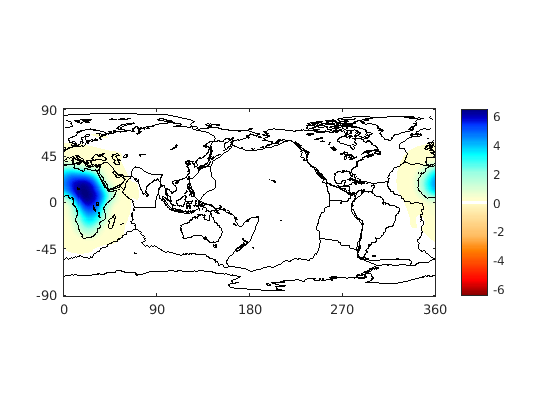
\includegraphics[width=0.5\textwidth]{figures/G(:,1)flatml.png}
  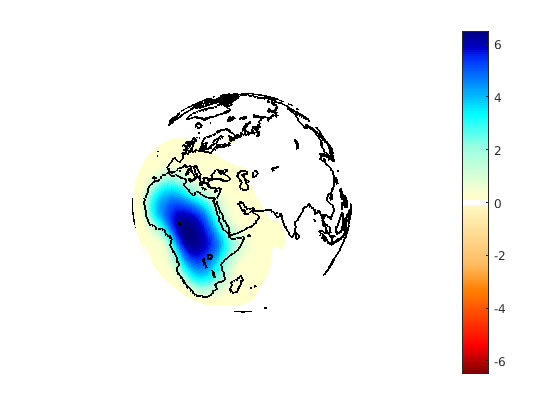
\includegraphics[width=0.45\textwidth]{figures/G(:,1)ml.png}
  \caption{Plot of G(:,1).}
\label{G(:,1)}
\end{figure}
Let's now use the function \verb+potup+ to upward continue the Slepian functions to satellite altitude.  We can now run:

\verb+coef = potup(G(:,1),rnew,rold,L,0);+

providing the output of the spherical harmonic coefficient vector for radial field at the new altitude.  We need to convert this to lmcosi format:

\verb+lmcosi = coef2lmcosi(coef,1);+

We can plot the functions at the satellite altitude.  To plot on a flat surface, run:

\verb+data = plm2xyz(lmcosi,res);+\\
\verb+plotplm(data,[],[],4,res)+\\
\verb+caxis([-1,1]*max(abs(caxis)))+\\
\verb+kelicol(1)+

To plot on a sphere, run:

\verb+plotplm(lmcosi,[],[],2,res)+

For the results, see figure 2.
\begin{figure}[H]
  %\centering
  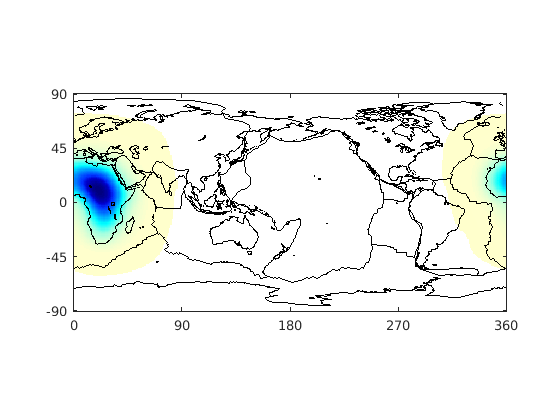
\includegraphics[width=0.5\textwidth]{figures/potupflatml.png}
  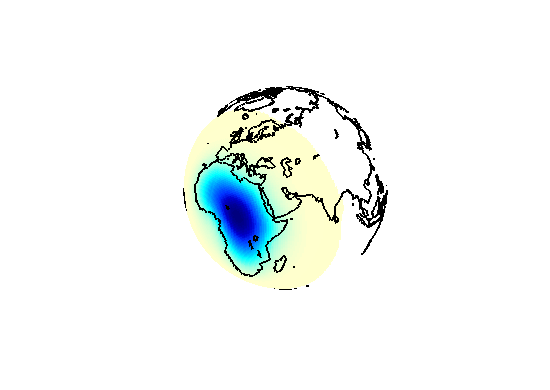
\includegraphics[width=0.45\textwidth]{figures/potupml.png}
  \caption{Upward continued G(:,1).}
\label{G(:,1)potup}
\end{figure}

\textbf{Exercise:} Let's try another region, say a spherical cap:

\verb+dom = [16]+

Run every step above again and plot on a sphere.  What is the result?  Compare your result to figure 3.

\textbf{Exercise:} We can try another region, say a spherical ring:

\verb+dom = [100,25]+

What is the result? Compare to figure 3.
\begin{figure}[H]
  \centering
  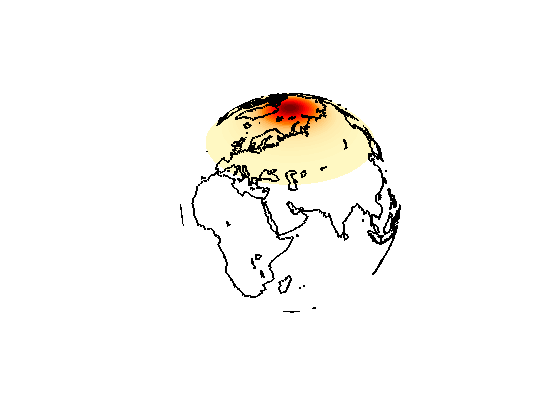
\includegraphics[width=0.45\textwidth]{figures/dom16ml.png}
  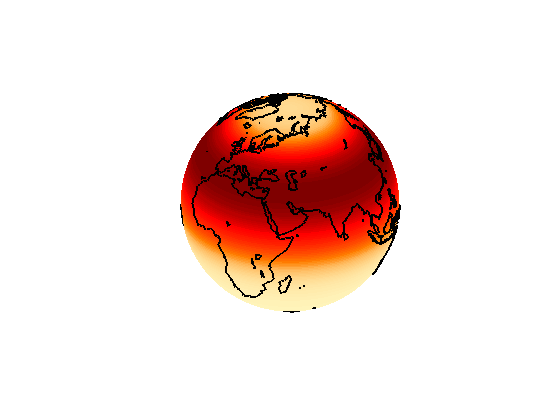
\includegraphics[width=0.45\textwidth]{figures/dom100_25ml.png}
  \caption{Result with dom = 16 and dom = [100,25]}
\label{dom}
\end{figure}
See the \verb+help+ function to see what other regions we can choose for \verb+glmalphapotup+.

\textbf{Exercise:} Try the second best Slepian function, now in Africa:

\verb+dom = 'africa';+\\
\verb+[G,V] = glmalphapotup(dom,L,rnew,rold);+\\
\verb+coef = potup(G(:,2),rnew,rold,L,1);+\\
\verb+lmcosi = coef2lmcosi(coef,1);+\\
\verb+plotplm(lmcosi,[],[],2,res)+\\
\verb+kelicol(1)+

This results in figure 4.  Compare with figure 2.  What do you notice?

\begin{figure}[H]
  \centering
  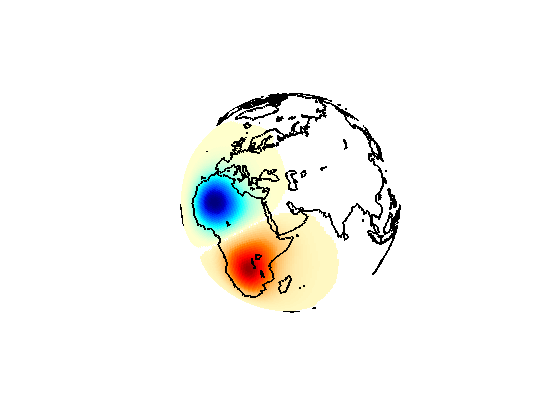
\includegraphics[width=0.45\textwidth]{figures/G(:,2)ml.png}
  \caption{Plot with the second best Slepian function, G(:,2).}
\label{G(:,2)}
\end{figure}

\subsection{Linear combinations of Slepian functions}

Now that we know how to create and plot the Slepain functions at satellite altitude with different regions, we can create a linear combination of the altitude-cognizant Slepian functions.  What does the linear combination 

\verb|h = G(:,1)+G(:,2);| 

look like?  You will need to input this linear combination into your command line and run the same process, with \verb+h+ instead of \verb+G(:,1)+ in the functions:

\verb+coef = potup(h,rnew,rold,L,1);+\\
\verb+lmcosi = coef2lmcosi(coef,1);+\\
\verb+plotplm(lmcosi,[],[],2,res)+\\
\verb+caxis([-1,1]*max(abs(caxis)))+\\
\verb+kelicol(1)+

This should result in figure 5.  Compare this figure with figures 2 and 4.  What do you notice?

\textbf{Exercise:} Try some of your own linear combinations and examine the plots.

\begin{figure}[H]
  \centering
  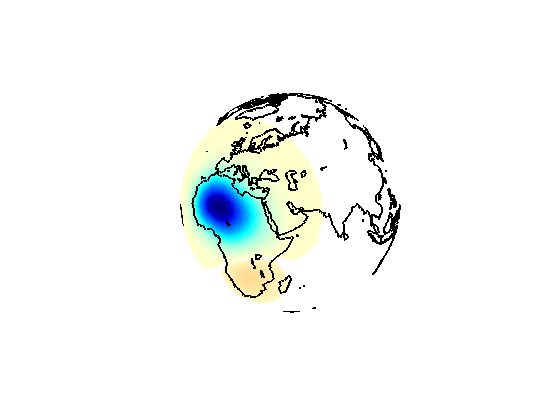
\includegraphics[width=0.5\textwidth]{figures/hcombml.png}
  \caption{Plot with h = G(:,1)+G(:,2).}
\label{lincomb1}
\end{figure}


\subsubsection{Example Two:}
Now, let's try a set of linear combinations including all of the spherical harmonic coefficients in our case.  The length of our matrix, G, is $(L+1)^2$.  Let:

\verb|K = length(G)|

We need to determine a proper value for \verb+J+ to plot the optimal linear combination of Slepian functions.  We will first need to plot our index \verb+j+ versus \verb+V+:

\verb|plot(1:K,V)|

Now we can analyze the plot to determine which value of J such that most of the eigenvalues are concentrated within our region.  Our plot will look like figure 6, as an exponential decay curve.  

\begin{figure}[H]
  \centering
  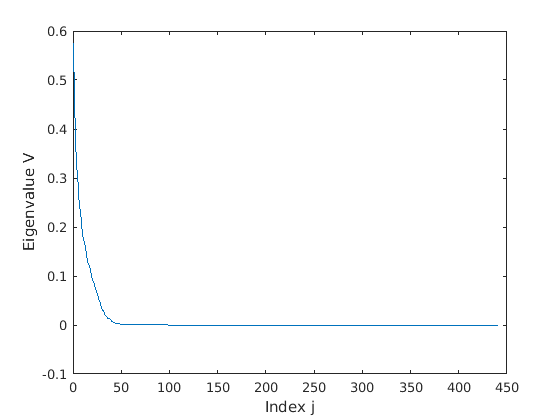
\includegraphics[width=0.5\textwidth]{figures/Vvsj_ml.png}
  \caption{Eigenvalue V vs index j.}
\label{lincomb}
\end{figure}

By analyzing the graph, it looks like the eigenvalues near zero at about $J=50$.  You will have to manually choose your J value, so run:

\verb+J = 50;+

We want to choose some random values to create our linear combination:

\verb|u = randn(K,1);|

and we will need to create a a matrix, \verb+f+, which is the same size as our coefficients. Run:

\verb|f = zeros(size(G(:,1)));|

Now we can make a \verb|for| loop to create a linear combination of the coefficients by running:

\verb|for j=1:J|\\
\verb|	f = f + u(j)*G(:,j);|\\
\verb|end|

This will create a matrix, \verb|f|, containing the linear combinations of spherical harmonics.  Now we can sort them into the correct format and plot:

\verb|[F,lon,lat] = plm2xyz(coef2lmcosi(f,1),1);|\\
\verb|plotplm(F,lon,lat,4,res)|

The plot of F is shown in figure 7.  We can alternatively directly plot this by:

\verb|plotplm(coef2lmcosi(f,1),[],[],4,res)|

\begin{figure}[H]
	\centering
	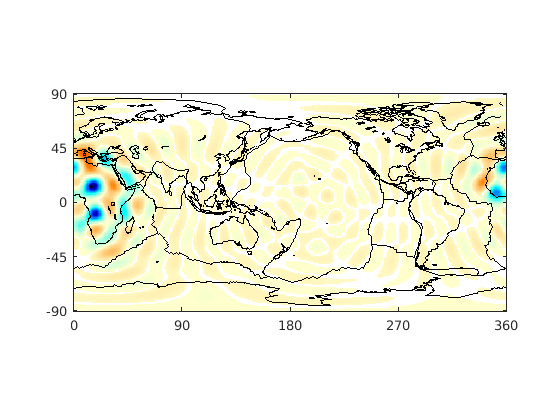
\includegraphics[width=0.5\textwidth]{figures/F_ml.png}
	\caption{Random linear combination for eignenvalues up to J = 50.}
\end{figure}


Now, let's use all of the Slepian functions, rather than just up to our value \verb|J|.  To do this, let's run a similar code with eigenvalues \verb|1:K|.

\verb|f2 = zeros(size(G(:,1)));|\\
\verb|for j=1:K|\\
\verb|	f2 = f2 + u(j)*G(:,j)|\\
\verb|end|

Plot:

\verb|plotplm(coef2lmcosi(f2,1),[],[],4,res)|

Figure 8 shows the plot of all of the eigenvalues.

\begin{figure}[H]
	\centering
	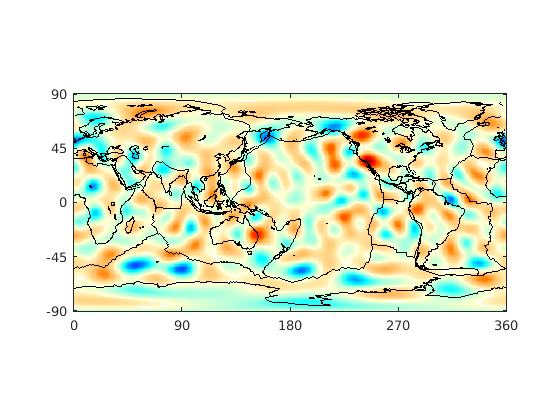
\includegraphics[width=0.5\textwidth]{figures/f2ml.png}
	\caption{Random linear combination for all eignenvalues.}
\end{figure}


Now that we understand the building of the linear combinations, we can use \verb|potup| to upward continue the coefficients.  We want to use our original \verb|f|, since it would be the best linear combination of Slepian functions.  We can do this in one step:

\verb|fup = potup(f,rnew,rold,L,1);|

Now we can plot the upward continued coefficients:

\verb|plotplm(coef2lmcosi(fup,1),[],[],4,res)|

The best fit Slepian functions, upward continued, are shown in figure 9.

\begin{figure}[H]
	\centering
	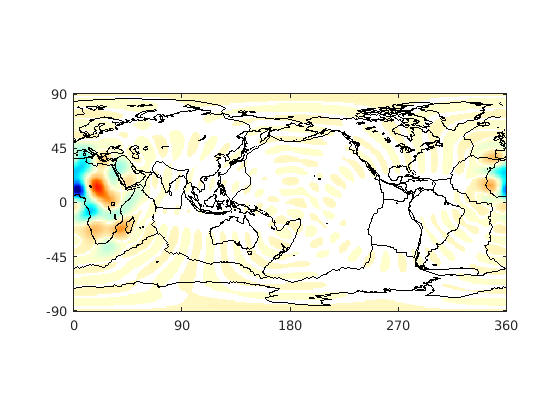
\includegraphics[width=0.5\textwidth]{figures/fup_ml.png}
	\caption{Best linear combination of Slepian functions up to J = 50, upward continued.}
\end{figure}

\textbf{Question:} Choose a lower J value and compare the plots.  What do you notice?


\TAG

\end{document}